\section{Stability Detector}
\label{sec:StabilityDetector}

A steady, stable system state is an obvious prerequisite for activating the electromagnet to pickup the puck and deactivating it to release the puck for reliable system performance.
A Simulink block diagram showing the stability detector may be seen in Figure \ref{fig:simulinkstability}.
Both speed and position are checked against experimentally established thresholds.
As previously discussed, the speed signal must be passed through a low pass filter. 
The pre-filtered signal is also checked in an effort to eliminate phase shift error caused by the filter.

\begin{figure}[htp]
    \centering
    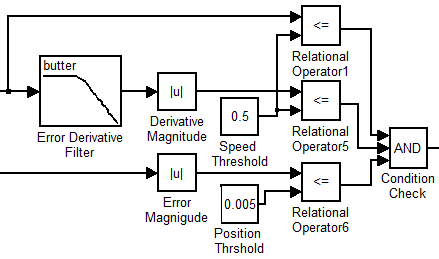
\includegraphics[scale=0.75]{images/StabilityDetector.PNG}
    \caption{Stability Detection}
    \label{fig:simulinkstability}
\end{figure}
